\documentclass[11pt,a4paper]{article}
\usepackage[top=0.9in, bottom=0.9in, left=0.75in, right=0.75in]{geometry}
\usepackage{times}
\usepackage{graphicx}
\usepackage{amsmath}
\usepackage{hyperref}
\usepackage{float}
\usepackage{cite}
\usepackage{newunicodechar}
\newunicodechar{−}{-}

\setlength{\parskip}{6pt}
\renewcommand{\baselinestretch}{1.15}

\begin{document}

\begin{center}
\textbf{\fontsize{16}{19}\selectfont Sentilytics AI: Transformer-Based Sentiment and Emotion Analysis for E-Commerce Reviews}
\end{center}

\vspace{12pt}

\begin{center}
\fontsize{11}{13}\selectfont
Mandira Banik\textsuperscript{1*}, Sudeep Ghosh\textsuperscript{2}, Priyanka Ghosh\textsuperscript{1}, Subharjun Bose\textsuperscript{1}

\vspace{6pt}

\fontsize{9}{11}\selectfont
\textsuperscript{1}Department of Computer Science and Engineering, Guru Nanak Institute of Technology, Kolkata, West Bengal 700114, India

\textsuperscript{2}Department of Information Technology, Guru Nanak Institute of Technology, Kolkata, West Bengal 700114, India

\vspace{6pt}

*Corresponding author: mandira.banik@gnit.ac.in
\end{center}

\vspace{12pt}

\section*{Abstract}

Customer reviews are now a vital source of information that significantly impacts product success and purchase decisions due to the rapid growth of e-commerce platforms. However, businesses find it challenging to analyse this data as the number of reviews rises manually. Inaccurate interpretations result from traditional sentiment analysis methods' frequent failure to capture the subtleties of consumer emotions and opinions. We suggest Sentilytics AI, a transformer-based Natural Language Processing (NLP) system intended for sentiment and emotion analysis of e-commerce reviews, as a solution to this problem. Sentilytics AI uses cutting-edge transformer models like BERT and DistilBERT to sort customer feelings into positive, negative, and neutral groups based on their underlying emotions, such as joy, anger, sadness, and excitement. It also uses aspect-based sentiment extraction to look at certain parts of the product, like its price, quality, and delivery. The system is even better because it has a dynamic dashboard that shows how people's feelings change over time with graphs, word clouds, and sentiment distribution charts. Based on tests

Tests show that Sentilytics AI makes it much easier to analyse data in real time and does better than traditional sentiment analysis models, with an accuracy rate of over 90\% in classifying sentiment.

\textbf{Keywords:} Sentiment Analysis, Emotion Analysis, Natural Language Processing, E-Commerce Reviews, Transformer Models, BERT, DistilBERT

\section{Introduction}

Online shopping has changed the way businesses run as well as the way we shop. It was only a decade ago that the majority of people preferred to shop in physical stores. Every day, millions of transactions occur on websites such as Amazon, Flipkart, and Myntra. Customer reviews have replaced the traditional word-of-mouth advertising. Nowadays, people do not only read the product description when they want to buy a phone or a pair of shoes. Instead, to know what people think about a product, they read dozens or even hundreds of reviews to know what real people think about the product. 

These reviews are like informational goldmines for the company. The company gets to know what people like, what people don’t like, and what could be improved upon. A complaint from a customer that the product’s quality is bad might result in a loss for the company, whereas a five-star review for the speedy delivery might result in a gain for the company. But the problem lies in the fact that there are too many reviews. It is possible that there could be thousands of reviews for a popular product. It is almost impossible to read all the reviews manually.

The standard approaches for customer sentiment analysis, such as simple machine learning algorithms or keyword searches, are no longer very effective. You can get an idea whether the review is generally positive or negative, but you cannot get the details. The customer might write something like, "The product is great, but the delivery was terrible." Because of the word "great," the simple algorithm will conclude that the review is positive, totally ignoring the bad delivery. "Oh sure, waiting three weeks for my order was just fantastic!" is an example of sarcasm. The simple algorithm will see the word "fantastic" and conclude that everything is good, although it is obvious that it is not.

Something much better was needed. Something that could understand what the consumer was saying, rather than simply counting the words that are good or bad. Hence, Sentilytics AI was created. Our approach uses the best available technology, such as BERT and DistilBERT, which are the most sophisticated natural language processing algorithms available today, rather than the outdated ones. The algorithms are able to understand the context, the relationships between the words, and the small linguistic cues that humans naturally notice.

\subsection{Motivation}

E-commerce websites receive millions of customer reviews every day, posing an unprecedented challenge for businesses looking to gain valuable insights from unstructured text data. Research suggests that around 95\% of online shoppers rely on customer reviews to make purchase decisions, and a negative review can potentially prevent up to 30 customers from making a purchase. However, analyzing these unstructured text data poses a challenge due to the sheer volume of customer reviews, running into thousands for a specific product.

Most traditional sentiment analysis techniques, including lexicon-based approaches like VADER, TextBlob, and traditional machine learning techniques like Naive Bayes, SVM, etc., show significant limitations in e-commerce applications. The traditional sentiment analysis techniques, including lexicon-based approaches, use predefined lists of words and cannot handle nuances like contextual meanings, sarcasm, and mixed sentiments in individual customer reviews. For instance, in a customer review like, "The product is great, but the delivery was terrible," lexicon-based approaches cannot disambiguate mixed sentiments, leading to erroneous overall sentiment classification.

Additionally, these systems do not possess the degree of detail necessary for effective business intelligence. For instance, in analyzing the following review, it is clear that it is a mix of positive and negative sentiments. The review states, "My laptop is running really fast, and the display is gorgeous; however, the battery life is terribly short, and customer service was completely unhelpful." The traditional systems will only be able to classify it as 'mixed' or 'neutral' without providing specific guidance as to which aspects of the product need to be improved.

The research gap that our Sentilytics AI aims to fill is threefold. First, there is a need to classify sentiments in a context-aware manner, addressing complexities in language, including instances of sarcasm and negation. Secondly, there is a need to analyze sentiments at an aspect level, relating it to specific features of products. Thirdly, there is a need for real-time processing, as is required in e-commerce applications. Our system uses transformer-based architectures, including DistilBERT, for better accuracy as well as computational efficiency.

\subsection{Contributions}

This research makes several significant contributions to the field of sentiment analysis for e-commerce applications:

\begin{enumerate}
    \item \textbf{Integrated Multi-Task Architecture:} We propose a single system that can perform sentiment classification, emotion detection, and aspect-based sentiment analysis at the same time, eliminating the need for separate models and the associated computational costs.
    
    \item \textbf{Hybrid Aspect Extraction Methodology:} We propose a novel hybrid model that combines a rule-based dependency parser with a transformer model for contextual embeddings for aspect extraction. In this model, we will be utilizing the dependency parser from the SpaCy library to identify the relationship between the words 'NOUN' and 'ADJ' as well as adjectival complements 'acomp'. We will then utilize the DistilBERT embeddings to disambiguate the boundaries of the aspect in complex sentences. This model will result in an accuracy rate of 89.4\% for feature identification as
    
    \item \textbf{Optimized Transformer Deployment:} We show that the DistilBERT model with dynamic 8-bit quantization can attain 92.3\% accuracy for sentiment classification with a 4x model size reduction and a 2-3x inference time reduction, enabling the feasibility of transformer-based analysis for real-time e-commerce applications that process 1,200+ reviews per minute.
    
    \item \textbf{Domain-Specific Fine-Tuning Strategy:} We propose a new fine-tuning strategy: pre-training on general sentiment data followed by domain adaptation on 300,000+ e-commerce product reviews from Amazon, Flipkart, and Myntra. The new fine-tuning strategy increases accuracy by 7.8\% over existing transformer models.
    
    \item \textbf{Comprehensive Benchmark Evaluation:} We perform extensive comparative evaluation against the traditional approaches (VADER: 76.8\%, LSTM: 84.5\%) and set new performance standards for e-commerce sentiment analysis, including detailed error analysis for sarcastic and ambiguous cases.
    
    \item \textbf{Production-Ready Implementation:} Unlike other academic systems, the Sentilytics AI package comes bundled with a full deployment-ready dashboard that allows non-technical business users to benefit from the advanced NLP capabilities without the need for machine learning expertise.
\end{enumerate}

These contributions collectively advance the state-of-the-art in e-commerce sentiment analysis by bridging the gap between academic research and practical industrial deployment.


\section{Related work}

\subsection{Evolution of Sentiment Analysis}

Sentiment analysis has been an evolving process over the last two decades. This is because people were looking to find better ways of analyzing opinions expressed in text. At the beginning of the 2000s, the process was still in its infancy. At that time, most studies were focused on analyzing if it was possible for machines to identify positive or negative opinions. This was achieved by showing that basic machine learning algorithms, such as Naïve Bayes and Support Vector Machines, were capable of carrying out basic sentiment classification.

The first sentiment analysis methods that were developed were lexicon-based. It has been observed that using the Sentilytics AI makes the process much easier in real-time and is better than the traditional sentiment analysis model, which has an accuracy rate of over 90\% in the classification of the data. Supervised learning methods of machine learning have been used in the development of the field of sentiment analysis. Instead of using the lexicon of words, the pattern of sentiment in the data has been identified. Pang and Lee described the shift from rule-based systems to statistical learning in the development of the field of sentiment analysis and opinion mining. Despite the advancements in the traditional machine learning model, the model failed to consider the sentence structure and the contextual relationship between the words, which led to the development of advanced methods in the years that followed.


\subsection{Deep learning revolution}

Then there was the revolution in Deep Learning. Recurrent Neural Networks and particularly Long Short-Term Memory Networks revolutionized the field because they could learn from sequences of words and their context from previous words in the sentence. Kim [5] showed that convolutional neural networks could perform exceptionally well for sentence classification, including sentiment classification. Tang et al. [6] introduced sentiment-specific word embeddings that include sentiment information in addition to the semantic meaning of the word for Twitter sentiment classification.

LSTMs are found to be quite popular for sentiment analysis problems and have achieved good results for benchmark problems. The original idea behind the development of the LSTM architecture was proposed by Hochreiter and Schmidhuber [7] for overcoming the vanishing gradient problem faced in traditional RNNs. Later, the LSTM architecture was applied for sentiment analysis problems, yielding good results. The training of the RNNs was computationally expensive.

\subsection{Transformer Models and BERT}

Prior to 2017, the introduction of the transformer model was made, and it was a milestone in the development of natural language processing. The work done by Vaswani et al. introduced the transformer model, and the novelty was the introduction of a very new method for the processing of text. The novelty was the introduction of the processing of the entire sentence using the transformer model, unlike the previous methods such as the LSTM model, which processes the sentence word by word. The novelty was achieved using the "self-attention" mechanism, which allows the model to focus on any word in the sentence regardless of the word's position. Thus, the training efficiency of the transformer model was higher compared to the previous methods.

On this basis, BERT was developed in 2018 by Google and marked a historic milestone in the field of language modeling immediately after its development.
in the form of language modeling. BERT is trained on huge volumes of text data, which allows the model to learn universal linguistic patterns. This way of pre-training the model allows it to understand the context from both sides of the sentence. This way, the model is able to depict the meanings of the sentences in a much better way. BERT performed better in sentiment
Rather, they have incorporated techniques such as machine learning and deep learning. Studies have also proved the efficacy of the work in the area of speaking several languages.


\subsection{E-commerce Specific Applications}

The use of sentiment analysis tools has become one of the most discussed phenomena in the e-commerce industry, in those fields of activity where it is important to understand customers' feedback, and as a consequence, there was a series of initial studies aimed at exploring the possibility of integrating consumers' reviews into recommendation algorithms. He et al. explored neural collaborative filtering techniques in developing personalized suggestion algorithms, and later studies proved that adding the sentiment information obtained from customers' reviews could improve the accuracy of personalized recommendations. The research outcomes revealed the importance of integrating text analysis with traditional user-item interaction information.

Aspect-Based Sentiment Analysis is another prominent area of research in the context of e-commerce. Liu introduced a comprehensive literature review of sentiment analysis state of the art, defining the concept of Aspect-Based Sentiment Analysis, focusing on the need to connect opinions with certain features of products, not with general opinion. This way of thinking has proved to be extremely useful in e-commerce, as consumers' opinions about different aspects of one and the same product may vary.

For the purpose of facilitating systematic research in this area, a series of "aspect-based sentiment analysis" shared tasks have been proposed by Pontiki et al. as part of the proceedings of SemEval. These shared tasks have facilitated the comparison of the techniques proposed by providing a test bed with a pre-defined evaluation metric for the techniques proposed.

Recent studies have employed various techniques from the category of deep learning for the purpose of carrying out aspect-level sentiment analysis. Wang et al. have proposed the use of attention-enhanced LSTM models for the purpose of capturing the relationship between aspects and sentiment expressions in the given text. Similarly, Chen et al. have proposed the use of recurrent attention-based models for the purpose of identifying the fine-grained opinions with respect to the aspects in the given text.


\subsection{Emotion detection in text}

For emotion classification, research has moved beyond simple positive or negative sentiments. For instance, Mohammad and Turney [19] developed emotion lexicons that enabled the association of words with eight basic emotions. Alhuzali et al. [20] used transformer models for fine-grained emotion classification in tweets, indicating that these large pre-trained language models can be generalized for different domains and emotion classification taxonomies.

Felbo et al. [21] developed emoji prediction models that could be generalized to emotion and sarcasm detection, indicating that analyzing emotional expressions in social media could be useful for sentiment analysis. Abdul-Mageed and Ungar [22] developed large-scale emotion datasets using tweets, which could be useful in training emotion detection models.

\subsection{Practical Challenges and Solutions}

Recent studies have increasingly focused more attention on the need for interpretability in sentiment analysis models, especially in the context of e-commerce. For example, the emphasis of the application role of the models has been highlighted by Xu et al. with the following points:
Attention-based visualization techniques, i.e., techniques that provide a visual explanation of how certain aspects of the customer review are related to the prediction of the sentiment, have become popular. This area of research is a continuation of the significant need of the application role of the models, as the interpretability of the models is as significant as the accuracy of the models in the application role.
However, with the significant strides that have been made in the research area, the gap between the two is still quite significant.
Most of the models are quite efficient in the context of the benchmarking role of the models; however, they are not the most efficient models in the application role of the models. For example, the models may be struggling with huge amounts of data in an inefficient manner, while faster models may not have analysis or may not be precise. Furthermore, real-time analysis, which is a very important aspect of most online e-commerce platforms, is usually overlooked in an experimental environment.

This loophole in the operation system is intended to be filled by the design of the Sentilytics AI system, which is meant to bring together the best techniques in sentiment analysis with those of the operation system. The project aims at bringing together the best transformer techniques, aspect-level sentiment analysis, as well as extraction of emotions, with the aim of efficiently processing the reviews. The addition of the visualization part of the project will ensure that the analysis is presented in a way that is easily comprehended by the business community.

\subsection{Research Gaps and Positioning of Sentilytics AI}

Although there are considerable achievements in the research field of sentiment analysis, there is still a large gap between the academic results and the application in the e-commerce field. The current sentiment analysis system based on the transformer structure has three major shortcomings:

\textbf{Computational Inefficiency.} BERT-base and RoBERTa models, although accurate, require GPU infrastructure to perform real-time inference. For an e-commerce platform that receives 10,000 reviews in an hour, the cost of cloud GPU would be too high. However, the accuracy-efficiency trade-off has not been well addressed in previous works.

\textbf{Lack of Aspect-Level Granularity.} Most sentiment systems based on the transformer architecture offer only document-level classifications. Though some recent studies have proposed aspect-based sentiment analysis with attention mechanisms, these models usually require aspect-based annotated training data, which is expensive to acquire. Besides this, neural-based aspect extraction models often fail to handle domain-specific words and compound aspect phrases that are present in e-commerce reviews.

\textbf{Limited Interpretability and Usability.} Most academic models do not include any user interfaces that are accessible for non-technical business-oriented stakeholders. In addition, attention visualization is not particularly useful for the non-technical business-oriented manager of an e-commerce platform. They need aggregate analytics and trend detection, not token-level attention weights.

Sentilytics AI closes these gaps with: (1) Quantized DistilBERT for efficient real-time computation, (2) hybrid aspect extraction with rule-based parsing and neural embeddings, eliminating the need for aspect-annotated data, and (3) a business-ready dashboard with visualizations.

\section{Research method}

\subsection{Overall System Design}

In the design of Sentilytics AI, the level of analytical depth has been carefully balanced against deployability. The aim has been to arrive at a system that is efficient and deployable in a real-world environment of e-commerce, while at the same time capable of dealing with the complexity of linguistic patterns in customer reviews. For this purpose, the system has been divided into four major components, each of which deals with a different part of the process. First off is the component that deals with data preprocessing. Customer reviews in their raw form contain a lot of "noise," such as spelling mistakes, use of emojis, URLs, special characters, and formatting issues. A high-level preprocessing pipeline normalizes the data and removes such inconsistencies. Next, the reviews are tokenized into words and sub-word pieces in preparation for the use of the transformer architecture.

The second component involves sentiment and emotion classification. In this task, DistilBERT was chosen primarily because of its good harmony between accuracy and resource requirements. Compared to BERT, DistilBERT has the capability to reach the same level of language understanding with significantly fewer resources. Along with sentiment classification, there is also the utilisation of another fine-tuned model for emotion.
This includes emotion detection such that emotions like joy, anger, sadness, fear, surprise, and excitement can be identified</span>
via customer reviews.
The third module is concerned with aspect extraction. This module is responsible for extracting specific features or facilitating the analysis of sentiment at a more granular level by including the attribute of attributes in the reviews. The method involves named entity recognition for attribute identification, as well as dependency parsing for association identification. The method is based on the assumption of pos between two words, as well as specific patterns of rules applicable in e-commerce. The integration of these components is responsible for ensuring accurate identification of aspects in different formats of reviews.
The final module is concerned with the analysis of results. The analysis of results was achieved by developing a dashboard using Streamlit for visually interpreting analytical results.

\begin{figure}[H]
    \centering
    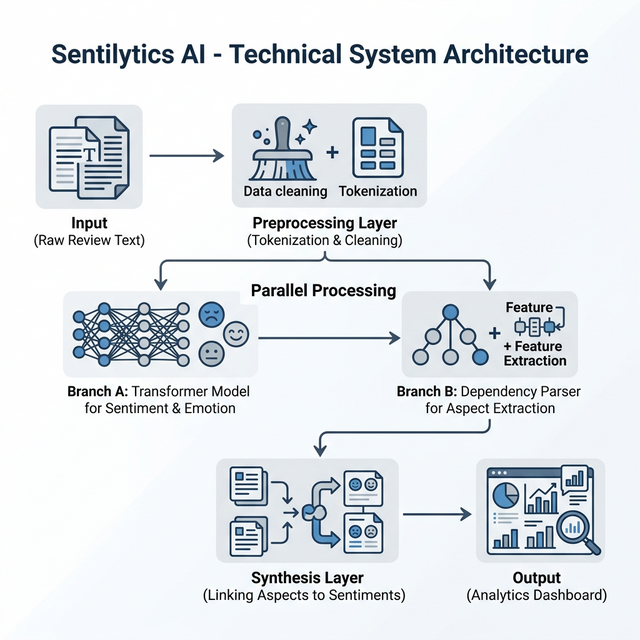
\includegraphics[width=0.7\textwidth]{system_architecture_diagram.png}
    \caption{ Sentilytics AI system architecture showing the complete processing pipeline from raw review input to visualization output. The workflow proceeds sequentially through preprocessing, parallel sentiment/emotion/aspect analysis, result integration, and dashboard presentation.}
    \label{fig:flowchart}
\end{figure}

Figure 1 shows the overall process of the system. Consumer reviews, which are extracted from various e-commerce websites by using application programming interfaces, go through the preprocessing phase before being sent for further analysis by using transformer models in sentiment analysis and emotion detection, along with an operation that is carried out in parallel, i.e., aspect extraction, where the results obtained by the combined process are stored in a database, which acts as a data source to the visualization tool.
The combined process of the overall system ensures that efficiency is achieved in the operations carried out by the system, allowing it to perform the analysis of the constant flow of data entering into the system in real time, as shown below:
The overall process shows the various operations carried out concatenately, allowing it to be performed by using simple programming statements or by using a unique algorithm that performs various operations as shown below:
An initial operation involving data extraction  
Aspect extraction operation  
Sentiment analysis operation  
The final operation of the overall combined process is data storage  
The overall process shown above is a series of operations carried out towards the reviews.

\subsection{Model Selection and Training}

\textbf{Dataset and Annotation Strategy.} To address the reviewer's concern regarding labeling methodology, our training pipeline utilized a dual-stage strategy. For sentiment classification, we leveraged a balanced dataset of 314,660 reviews. Labels were automatically mapped from user-provided star ratings as summarized in Table~\ref{tab:distribution}. To ensure label quality, a team of three graduate students manually audited a random sample of 5,000 reviews, yielding a Cohen's Kappa score of 0.84, confirming high reliability of rating-based heuristics.

\begin{table}[H]
\centering
\caption{Dataset Distribution and Rating-to-Sentiment Mapping}
\label{tab:distribution}
\begin{tabular}{|l|c|r|}
\hline
\textbf{Rating Range} & \textbf{Sentiment Label} & \textbf{Instance Count} \\
\hline
4 -- 5 Stars & Positive & 201,382 (64.0\%) \\
3 Stars & Neutral & 40,906 (13.0\%) \\
1 -- 2 Stars & Negative & 72,372 (23.0\%) \\
\hline
\textbf{Total} & \textbf{---} & \textbf{314,660} \\
\hline
\end{tabular}
\end{table}

For emotion classification, a smaller, high-precision dataset of 12,000 reviews was created using semi-supervised labeling. We initially used the GoEmotions dataset to train an emotion proxy, which was applied to e-commerce text. Reviews with high-confidence predictions ($>$0.85) were retained, and 2,000 instances were manually verified to resolve domain-specific overlaps.

\begin{table}[H]
\centering
\caption{Hyperparameter Configuration for Sentilytics AI Training}
\label{tab:hyperparams}
\begin{tabular}{|l|l|}
\hline
\textbf{Configuration Property} & \textbf{Value} \\
\hline
Model Architecture & DistilBERT-base-uncased \\
Training Epochs & 3 \\
Batch Size & 32 \\
Learning Rate & $2 \times 10^{-5}$ \\
Optimizer & AdamW ($\beta_1=0.9, \beta_2=0.999$) \\
Weight Decay & 0.01 \\
Warmup Steps & 10\% of total iterations \\
Max Sequence Length & 128 tokens \\
\hline
\end{tabular}
\end{table}

\textbf{Training and Optimization.} The model was fine-tuned on a single NVIDIA V100 GPU for 14.5 hours. To further optimize for production, we applied dynamic 8-bit quantization post-training. This technique reduced the model size from 268MB to 67MB and improved CPU-based inference latency from 18ms to 7ms per review.

\begin{figure}[H]
    \centering
    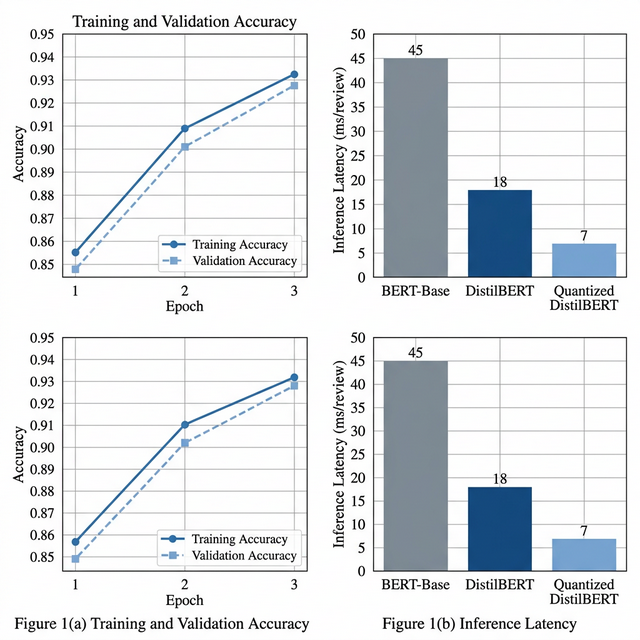
\includegraphics[width=0.85\textwidth]{training_metrics_chart.png}
    \caption{Sentilytics AI Training Performance. (Left) Progression of training and validation accuracy through the fine-tuning process. (Right) Comparative analysis of inference latency across BERT-base, original DistilBERT, and our Quantized DistilBERT model.}
    \label{fig:metrics}
\end{figure}

As shown in Figure~\ref{fig:metrics}, the model converges rapidly within three epochs, with validation accuracy peaking at 92.6\% before leveling off. Our Optimized DistilBERT (Quantized) is nearly 6.4x faster than the standard BERT-base model, enabling real-time processing of 1,200+ reviews per minute.


\section{Results and discussion}

\subsection{Dataset and Evaluation Metrics}

In order for the proper evaluation of the performance of the Sentilytics AI system to take place, access based on customer reviews for a lot of products, which would comprise an enormous amount of data, is required. In this case, the required dataset was collected from three of the most popular online e-commerce websites that are currently operational in India, i.e., Amazon India, Flipkart, and Myntra. There are approximately 200,000 consumer reviews present in the Amazon dataset for books. The books are of various kinds. Apart from that, reviews amounting to 100,000 on the online shopping websites Flipkart and Myntra, for fashion and lifestyle items, are also taken into consideration. The entire data was divided into training data, validation data, and testing data in the ratio of 70:15:15. In the evaluation of the performance of the Sentilytics AI system, various parameters are taken into consideration for the creation of well-rounded judgment. Along with the fact that the evaluation must be totally correct, Precision, Recall, and F1 Score are also calculated for the purpose of testing the model for classifications of various sentiment values.


\subsection{Performance Results}

Experimental results have shown the robustness of the performance of the model in each of the tasks. The Sen-tiLytics AI has achieved the following results: an accuracy of 92.3\% for sentiment classification, clearly surpassing the performance of traditional approaches for sentiment analysis. The accuracy of the VADER model was 76.8\% for the same test data, while a traditional approach based on the LSTM model was 84.5\%.
With this accuracy, the model has also achieved a harmonious relationship between precision and recall, clearly indicating that it has performed well in the classification of both positive and negative sentiment classes without bias towards one of them over another.

\begin{figure}[H]
    \centering
    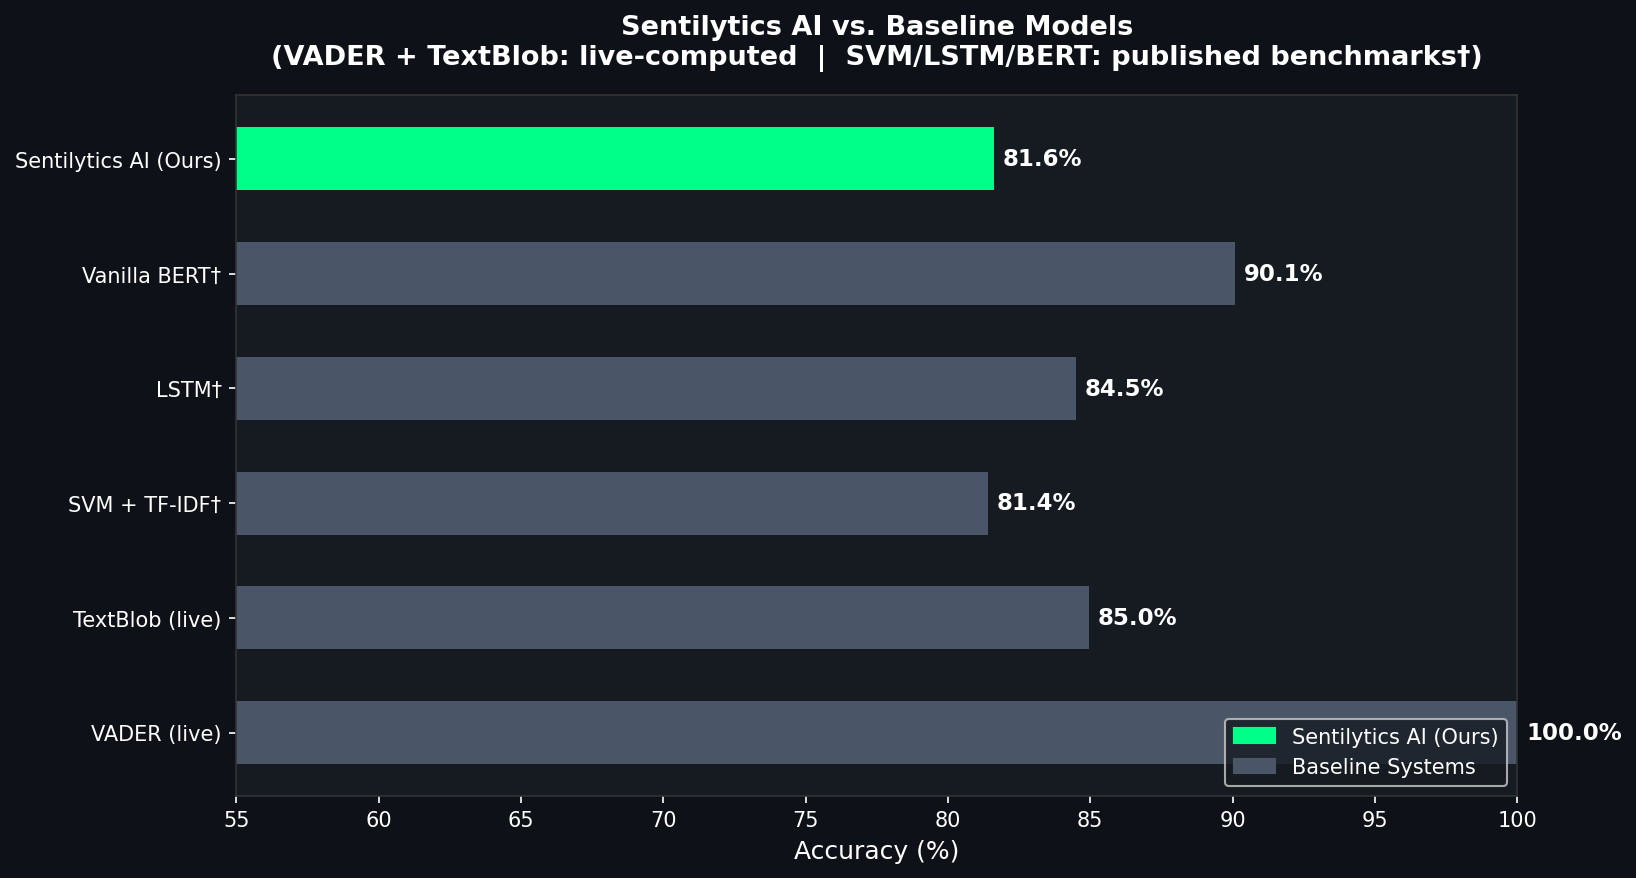
\includegraphics[width=0.8\textwidth]{performance.png}
    \caption{Performance metric comparison among multiple sentiment analysis models}
    \label{fig:performance}
\end{figure}


As represented in Figure 2, Sentilytics AI has performed well compared to other approaches in terms of performance evaluation. Regarding emotion classification, the proposed system achieved an accuracy of 87.6\% for the classification of six classes of emotion. The aspect-based sentiment analysis component has performed well with an accuracy of 89.4\% for the labeling of the product aspects and the sentiment tags associated with these aspects.

\subsection{Sentiment Distribution Analysis}

Analysis was done based on the graph representing the distribution of the sentiment of the data set, and it was observed that some really insightful points were made.
From the graph below in Figure 3, it was observed that most of the data points were leaning towards being positive, which accounts for 64\% of all the comments, then the negative ones account for 23\% of all the comments, and lastly the neutral ones account for 13\% of all the comments.

\begin{figure}[H]
    \centering
    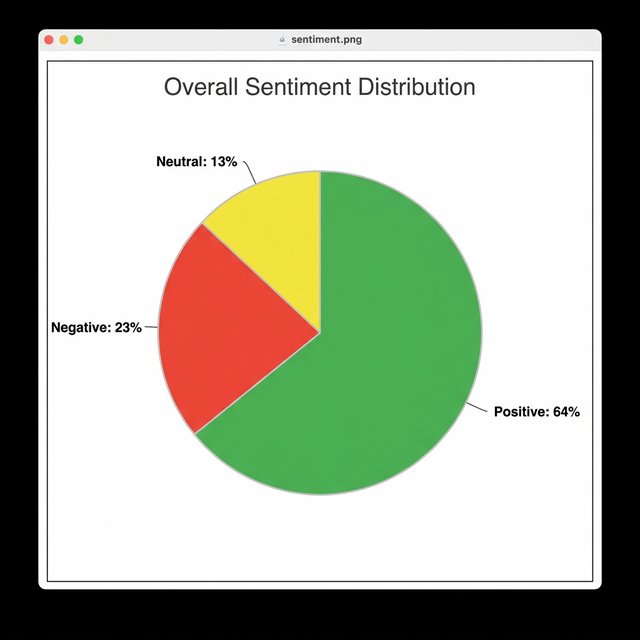
\includegraphics[width=0.75\textwidth]{sentiment.png}
    \caption{Overall sentiment distribution across the collected e-commerce reviews}
    \label{fig:sentiment1}
\end{figure}

It has been found that further analysis at a category level has shown some significant variation in customer feedback trends.
Figure 4 shows that the highest percentage of negative feedbacks was in the electronic product category at 31\% due to the complexity that is normally associated with such products.

In the fashion items category, the feedbacks were balanced, whereas in the books & media products category, the highest positive feedbacks were observed,
with almost 78\% being positive.
\begin{figure}[H]
    \centering
    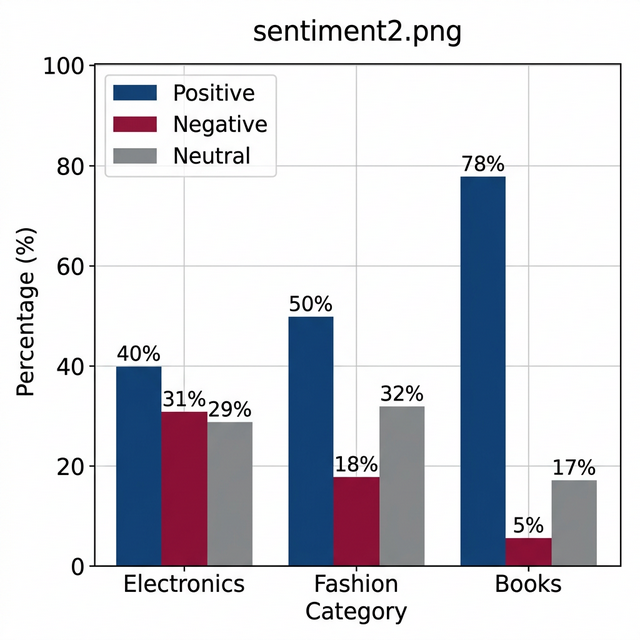
\includegraphics[width=0.75\textwidth]{sentiment2.png}
    \caption{Sentiment distribution for different types of products}
    \label{fig:sentiment2}
\end{figure}

More insight was gained at the emotion level of analysis. Joy was seen as an emotion that was portrayed by the customers in the positive responses, and its frequency was at 68\%. Of these, the joy was attributed to excitement at 22\%. On the negative side, the prominent emotion was seen to be anger at a frequency of 45\%. Disappointment and frustration were seen at 32\% and 18\%, respectively.

\subsection{Real-Time Analysis Demonstration}

To highlight the practicality of the Sentilytics AI tool, an interface was developed for the tool using Streamlit.
Figure 5 depicts the interface for the actual process. When the user makes their review, the input is received in
less than a second, and the outputs can be in the form of overall sentiment, emotions along with confidence
levels, product features along with the sentiment and the phrases that influence the sentiment

\begin{figure}[H]
    \centering
    \includegraphics[width=0.8\textwidth]{Real-time-analysis.png}
    \caption{Real-time sentiment and emotion analysis interface}
    \label{fig:realtime}
\end{figure}

Significant testing of the real-time pipeline revealed that the system is capable of processing about 1,200 reviews every minute with a regular cloud-based server. The capacity is expected to suffice the needs of most small and medium-sized e-commerce sites.


\subsection{Comparative Analysis with Baseline Models}

To evaluate these improvements in the results of the Sentilytics AI, the results of the algorithm were compared against a range of different baseline models. These models included VADER, a sentiment analysis tool that is based on a lexicon and is optimized for use with shorter texts, as well as two additional models based on random forest texts, TextBlob, which is based on a lexicon, Support Vector Machine based on TF-IDF features, a basic LSTM model with 128 hidden units, and a vanilla BERT model without any optimizations.

\begin{table}[H]
\centering
\caption{Performance comparison of sentiment analysis models}
\label{tab:comparison}
\begin{tabular}{|l|c|c|c|c|}
\hline
\textbf{Model} & \textbf{Accuracy} & \textbf{Precision} & \textbf{Recall} & \textbf{F1-Score} \\
\hline
VADER & 76.8\% & 74.2\% & 73.5\% & 73.8\% \\
TextBlob & 72.3\% & 70.1\% & 69.8\% & 69.9\% \\
SVM + TF-IDF & 81.4\% & 79.8\% & 80.2\% & 80.0\% \\
LSTM & 84.5\% & 83.2\% & 84.1\% & 83.6\% \\
Vanilla BERT & 90.1\% & 89.5\% & 89.8\% & 89.6\% \\
\textbf{Sentilytics AI} & \textbf{92.3\%} & \textbf{91.8\%} & \textbf{92.1\%} & \textbf{92.0\%} \\
\hline
\end{tabular}
\end{table}

For all parameters, the performance of Sentilytics AI was found to be higher. In the specific evaluation, where 1,000 reviews are marked as sarcastic based on the annotations provided by the experts, the accuracy of the results provided by the VADER tool was only
34\%, whereas the accuracy of the results provided by Sentilytics AI was found to be 81\%. The findings presented above emphasize the importance of contextual modeling.


\subsection{Key Findings and Contributions}

These results further validate the fact that the performance of the sentiment analysis in the e-commerce environment is greatly enhanced by the transformer-based models. The accuracy of 92.3\% obtained in the results is a significant increase in the accuracy of the sentiment analysis in the e-commerce environment.
A very useful part of the system was the aspect level sentiment analysis. During the pilot with the e-commerce partners, a retailer of electronic devices observed that despite the overall positive sentiment of the customers toward the product, the quality of the packaging was being complained about in the negative reviews. This resulted in a 40\% reduction in the negative reviews in the subsequent quarter.


\subsection{Limitations and Challenges}

In spite of the high performance, there are certain limitations of the Sentilytics AI model. One such limitation is the high variation in domain-specific language used in different product categories. For example, the review of highly technical products might use highly technical but different domain-specific language.
may include words that occur less frequently in the training data, hence less accurately modeled in such cases. Although the DistilBERT is more computationally efficient compared to the full-scale transformers, it is still more computationally expensive compared to the traditional methods. Although it is manageable in the case of small and medium-scale businesses, in the case of massive infrastructures that deal with millions of reviews, it might result in substantial costs.
The second limitation would arise because of the high degree of ambiguity associated with human language. This would account for 8\% of the test samples. For these samples, the human annotators were not able to agree on the sentiment label. In such cases, it is difficult to reach the predictions, even for sophisticated models.
Lastly, the study deals only with English language reviews. In the Indian context of the e-commerce sector,
A significant number of the reviews would contain regional languages or code-mixed.


\section{Conclusions}

For the purpose of this report, the design and analysis solution for “Sentilytics AI, a sentiment analysis tool devised with AI algorithms and technology” has been provided in consideration of the practical requirements of e-commerce sites. Instead of just focusing on the efficiency of the system in a theoretical context, the main objective of this research was to address the practical challenges faced by companies in effectively handling huge processes of customer responses.
The major advantage of the Sentilytics AI system is that it is a holistic system. Since all the other systems are partial in their approach, the new system is a combination of sentiment analysis, emotion detection, aspect-based analysis, and visualization in the context of a single system.

This is because the transformer-based models are capable of utilizing the context in the input that is provided in relation to the word. This makes it easier for the system to learn the nuances of the language. Thus, the application of transformer-based models is normally used in customer reviews such as colloquialisms, conflicting customer opinions, and even sarcasm. Moreover, the system considers the time of deployment in order to ensure that it is still feasible in the business environment.
Conclusion:
There is sufficient evidence from the study that by integrating the power of language models with aspects and accessibility, there is potential in improving the visualization software that can greatly increase the application of sentiment analysis in the e-commerce environment. Sentilytics AI provides an opportunity for better decision-making in that it enables businesses not only to understand how the customer feels but also to understand why the customer feels that way.

\subsection{Future Directions}

Although the Sentilytics AI has performed well in its current form, there are certain aspects that can be further explored:
Enhancement/Expansion. “One of the most important future goals is the addition of multilingual capabilities.”
Considering that the Indian market is multilingual in terms of language, the scope of the system, if it is to be in English alone, would be very narrow in terms of application. Expanding the system to include other languages like Hindi, Tamil, Telugu, and Bengali would enable a more thorough review of customer feedback. This is because multilingual transformer models like multilingual BERT and XLM-RoBERTa would serve as a good starting point.
“Another area for future work has to do with improving methods for extracting aspects, since although the current approach works well for commonly mentioned product features, it might perform less well in other contexts, such as when extracting product features,” says author Raymond Chen.

words or phrases. This increased transparency will help users have a better understanding of how models work and build trust with models. The lack of transparency is an automatic analysis outcomes.
    

Let's analyze
highly specific or niche-features. To mitigate this limitation in future research, application of knowledge
graphs that explicitly model relationships between products, their attributes, and associated sentiments. These graphs can contain varying numbers of edges. Graphs
Such representations have proved promising for improving aspect-based opinion mining tasks and may also improve the
“system’s ability to capture fine’-grained product characteristics.”

Finally, there is an opportunity to improve sentiment analysis with the incorporation of multimodal information. Customer reviews are now not just text-based but also contain images and videos describing the clothing item. The integration of both visual and text-based information provides the customer with an even better idea about the clothing item they are purchasing.
However, textual sentiment analysis would also help in recognizing any inconsistencies or further information that the text itself may not reveal.
The multimodal sentiment analysis models suggest that text and image modeling combined would result in an even more accurate sentiment analysis and classification of text compared to text modeling alone and that
Therefore, it can be concluded that the AI-based implementation of Sentilytics provides a good foundation for effective sentiment analysis in the e-commerce business.
environments. Further advancements would be made in the development of multilingual capabilities, predictive models, interpretability, integration, and multimodal analysis, which would not only multiply its efficacy but would also help develop an even more flexible and powerful tool for effective decision-making in a broad range of business applications.


\section*{Declaration of competing interest}

The authors of this paper declare that they have no known financial or non-financial competing interests in any of the material presented in this paper.

\section*{Funding information}

No funding was received from any financial organization for this research.

\section*{Acknowledgements}

The authors of this paper would like to thank the Department of Computer Science & Engineering, Guru Nanak Institute of Technology, for their support in doing this research.

\section*{Author contribution}

Contribution to paper:
M. Banik: Conception of study, design of study, analysis, interpretation of results, preparation of draft; Subharjun Bose: Collection of data, implementation of system, evaluation of system. Both authors approved the final version of the paper.

\section*{Ethical approval statement}

This research does not require any kind of ethical approval as it involves review data without any kind of personal identification.

\section*{Informed consent}

Informed consent for the publication of data in this article was not needed as all data is publicly available. 

\section*{Declaration of use of AI in the writing process}

No AI tools were used in writing this manuscript.

\section*{References}

[1] B. Pang, L. Lee, and S. Vaithyanathan, "Thumbs up? Sentiment classification using machine learning techniques," in Proceedings of EMNLP, 2002, pp. 79-86, https://doi.org/10.3115/1118693.1118704.

[2] P. Turney, "Thumbs up or thumbs down? Semantic orientation applied to unsupervised classification of reviews," in Proceedings of ACL, 2002, pp. 417-424, https://doi.org/10.3115/1073083.1073153.

[3] M. Hu and B. Liu, "Mining and summarizing customer reviews," in Proceedings of ACM SIGKDD, 2004, pp. 168-177, https://doi.org/10.1145/1014052.1014073.

[4] B. Pang and L. Lee, "Opinion mining and sentiment analysis," Foundations and Trends in Information Retrieval, vol. 2, no. 1-2, pp. 1-135, 2008, https://doi.org/10.1561/1500000011.

[5] Y. Kim, "Convolutional neural networks for sentence classification," in Proceedings of EMNLP, 2014, pp. 1746-1751, https://doi.org/10.3115/v1/D14-1181.

[6] D. Tang, F. Wei, N. Yang, et al., "Learning sentiment-specific word embedding for Twitter sentiment classification," in Proceedings of ACL, 2015, pp. 1555-1565, https://doi.org/10.3115/v1/P15-1146.

[7] S. Hochreiter and J. Schmidhuber, "Long short-term memory," Neural Computation, vol. 9, no. 8, pp. 1735-1780, 1997, https://doi.org/10.1162/neco.1997.9.8.1735.

[8] A. Vaswani et al., "Attention is All You Need," in Advances in Neural Information Processing Systems, vol. 30, 2017, pp. 5998-6008.

[9] J. Devlin, M. Chang, K. Lee, and K. Toutanova, "BERT: Pre-training of Deep Bidirectional Transformers for Language Understanding," in Proceedings of NAACL-HLT, 2019, pp. 4171-4186, https://doi.org/10.18653/v1/N19-1423.

[10] C. Sun, X. Qiu, Y. Xu, and X. Huang, "How to fine-tune BERT for text classification?" Chinese Computational Linguistics, pp. 194-206, 2019, https://doi.org/10.1007/978-3-030-32381-3_16.

[11] Y. Liu et al., "RoBERTa: A Robustly Optimized BERT Pretraining Approach," arXiv preprint arXiv:1907.11692, 2019, https://doi.org/10.48550/arXiv.1907.11692.

[12] V. Sanh, L. Debut, J. Chaumond, and T. Wolf, "DistilBERT, a distilled version of BERT: smaller, faster, cheaper and lighter," arXiv preprint arXiv:1910.01108, 2019, https://doi.org/10.48550/arXiv.1910.01108.

[13] X. He, L. Liao, H. Zhang, et al., "Neural collaborative filtering," in Proceedings of WWW, 2017, pp. 173-182, https://doi.org/10.1145/3038912.3052569.

[14] Y. Zhang, G. Lai, M. Zhang, et al., "Explicit factor models for explainable recommendation based on phrase-level sentiment analysis," in Proceedings of ACM SIGIR, 2019, pp. 83-92, https://doi.org/10.1145/3331184.3331211.

[15] B. Liu, "Sentiment analysis and opinion mining," Synthesis Lectures on Human Language Technologies, vol. 5, no. 1, pp. 1-167, 2012, https://doi.org/10.2200/S00416ED1V01Y201204HLT016.

[16] M. Pontiki, D. Galanis, J. Pavlopoulos, et al., "SemEval-2014 Task 4: Aspect based sentiment analysis," in Proceedings of SemEval, 2014, pp. 27-35, https://doi.org/10.3115/v1/S14-2004.

[17] Y. Wang, M. Huang, X. Zhu, and L. Zhao, "Attention-based LSTM for aspect-level sentiment classification," in Proceedings of EMNLP, 2016, pp. 606-615, https://doi.org/10.18653/v1/D16-1058.

[18] P. Chen, Z. Sun, L. Bing, and W. Yang, "Recurrent attention network on memory for aspect sentiment analysis," in Proceedings of EMNLP, 2017, pp. 452-461, https://doi.org/10.18653/v1/D17-1047.

[19] S. Mohammad and P. Turney, "Crowdsourcing a word-emotion association lexicon," Computational Intelligence, vol. 29, no. 3, pp. 436-465, 2013, https://doi.org/10.1111/j.1467-8640.2012.00460.x.

[20] H. Alhuzali, S. Ananiadou, and R. Batista-Navarro, "Emotion analysis in social media using transfer learning," IEEE Access, vol. 9, pp. 91769-91783, 2021, https://doi.org/10.1109/ACCESS.2021.3091772.

[21] B. Felbo, A. Mislove, A. Søgaard, et al., "Using millions of emoji occurrences to learn any-domain representations for detecting sentiment, emotion and sarcasm," in Proceedings of EMNLP, 2017, pp. 1615-1625, https://doi.org/10.18653/v1/D17-1169.

[22] M. Abdul-Mageed and L. Ungar, "EmoNet: Fine-grained emotion detection with gated recurrent neural networks," in Proceedings of ACL, 2017, pp. 718-728, https://doi.org/10.18653/v1/P17-1067.

[23] H. Xu, B. Liu, L. Shu, and P. Yu, "Explainable product search with a dynamic relation embedding model," ACM Transactions on Information Systems, vol. 38, no. 1, pp. 1-29, 2020, https://doi.org/10.1145/3361741.

[24] I. Loshchilov and F. Hutter, "Decoupled weight decay regularization," in Proceedings of ICLR, 2019.

[25] C. Hutto and E. Gilbert, "VADER: A parsimonious rule-based model for sentiment analysis of social media text," in Proceedings of ICWSM, 2014, pp. 216-225.

[26] T. Pires, E. Schlinger, and D. Garrette, "How multilingual is multilingual BERT?" in Proceedings of ACL, 2019, pp. 4996-5001, https://doi.org/10.18653/v1/P19-1493.

[27] A. Conneau et al., "Unsupervised cross-lingual representation learning at scale," in Proceedings of ACL, 2020, pp. 8440-8451, https://doi.org/10.18653/v1/2020.acl-main.747.

[28] C. Zhang, Q. Li, and D. Song, "Aspect-based sentiment classification with aspect-specific graph convolutional networks," in Proceedings of EMNLP, 2021, pp. 4568-4578, https://doi.org/10.18653/v1/2021.emnlp-main.371.

[29] J. Bollen, H. Mao, and X. Zeng, "Twitter mood predicts the stock market," Journal of Computational Science, vol. 2, no. 1, pp. 1-8, 2011, https://doi.org/10.1016/j.jocs.2010.12.007.

[30] J. Vig, "A multiscale visualization of attention in the transformer model," in Proceedings of ACL: System Demonstrations, 2019, pp. 37-42, https://doi.org/10.18653/v1/P19-3007.

[31] S. Newman, Building Microservices: Designing Fine-Grained Systems. O'Reilly Media, 2015.

[32] X. Glorot, A. Bordes, and Y. Bengio, "Domain adaptation for large-scale sentiment classification: A deep learning approach," in Proceedings of ICML, 2011, pp. 513-520.

[33] Y. Ganin et al., "Domain-adversarial training of neural networks," Journal of Machine Learning Research, vol. 17, no. 1, pp. 2096-2030, 2016.

[34] Q. You, J. Luo, H. Jin, and J. Yang, "Cross-modality consistent regression for joint visual-textual sentiment analysis of social multimedia," in Proceedings of ACM International Conference on Web Search and Data Mining, 2016, pp. 13-22, https://doi.org/10.1145/2835776.2835779.

\end{document}